\documentclass[a4paper,12pt]{article}

%%  Pacotes:
\usepackage{multirow}
\usepackage{graphicx}
\usepackage[table,xcdraw]{xcolor}
\usepackage[utf8]{inputenc}
\usepackage{amsmath, amsfonts, amssymb, latexsym, mathrsfs, amsthm, bezier, amscd}
\usepackage{soul}
\usepackage{caption}
\usepackage{subcaption}
\usepackage[french]{babel}
\usepackage{setspace}  
\usepackage{multicol}
\usepackage{cite}
\usepackage{url}
\usepackage{indentfirst}
\usepackage{multirow}
\usepackage{multicol}
\usepackage[final]{pdfpages}
\usepackage{indentfirst}
\usepackage{courier}
\usepackage[colorlinks,urlcolor=blue,filecolor=black,citecolor=black,linkcolor=black, pdfusetitle]{hyperref}
\usepackage{bookmark}
\usepackage{array, makecell} %
\usepackage{listings}
\usepackage[T1]{fontenc} 

\usepackage{amsmath}
\usepackage{enotez}
\setenotez{list-name=Notes de fin de document}
\DeclareInstance{enotez-list}{itemize}{list}{list-type=itemize}
\usepackage{titling}
\usepackage{float}
\usepackage{placeins}
\usepackage{lipsum}
\usepackage{esint}
\newcommand{\aspas}[1]{``#1''}
\usepackage{amsfonts}
\usepackage{amssymb}
\usepackage{wrapfig}
\usepackage{nicefrac}
\usepackage{mathtools}
\usepackage[per-mode=symbol]{siunitx}
\usepackage[ddmmyyyy]{datetime}
\usepackage[margin=1.0in]{geometry}
\usepackage{graphicx}
\usepackage{chngcntr}
\usepackage{xurl}
\usepackage{hyperref}
\usepackage{afterpage}
\usepackage{listings}
%\usepackage[table,xcdraw]{xcolor}
\usepackage{pgfplots}
\pgfplotsset{compat=1.15}
\usepackage{mathrsfs}
\usepackage{tikz}
\usetikzlibrary{arrows}
%\usepackage[top=3cm, bottom=3cm, left=3cm, right=2cm]{geometry}

\renewcommand\theendnote{\underline{\roman{endnote}}}
\renewcommand\thefigure{\thesection.\arabic{figure}}
\counterwithin{figure}{section}
\numberwithin{equation}{section}


\lstdefinestyle{mystyle}{
    backgroundcolor=\color{white},   
    commentstyle=\color{green},
    keywordstyle=\color{blue},
    numberstyle=\tiny\color{gray},
    stringstyle=\color{codepurple},
    basicstyle=\ttfamily\footnotesize,
    breakatwhitespace=false,         
    breaklines=true,                 
    captionpos=b,                    
    keepspaces=true,                 
    numbers=left,                    
    numbersep=5pt,                  
    showspaces=false,                
    showstringspaces=false,
    showtabs=false,                  
    tabsize=2
}
\lstset{style=mystyle}
%\usepackage[paper=portrait,pagesize]{typearea}


% Parâmetros:
\setlength{\parindent}{1.25cm}                       


\renewcommand{\j}{\ensuremath{j}}
\renewcommand{\ang}[1]{\ensuremath{\num{#1}^\circ}}
\newcommand{\eval}[2]{\left.#1\right|_{#2}}
\newcommand{\real}[1]{\Re\left\{#1\right\}}
\newcommand{\imag}[1]{\Im\left\{#1\right\}}
\newcommand{\op}[1]{\operatorname{#1}}
\newcommand{\pd}[3]{\frac{\partial^{#3} #1}{{\partial#2}^{#3}}}
\newcommand{\deriv}[3]{\frac{d^{#3} #1}{{d#2}^{#3}}}
\newcommand{\abs}[1]{\left\vert#1\right\vert}
\newcommand{\swr}{\operatorname{SWR}}
\newcommand{\ibv}{\hat{\mathrm{i}}}
\newcommand{\jbv}{\hat{\mathrm{j}}}
\newcommand{\kbv}{\hat{\mathrm{k}}}
\newcommand{\sen}{\operatorname{sen}}
\newcommand{\senh}{\operatorname{senh}}
\newcommand{\tg}{\operatorname{tg}}
\newcommand{\tgh}{\operatorname{tgh}}
\newcommand{\ita}{\textit}
\newcommand{\R}{\mathbb{R}}
\newcommand{\C}{\mathbb{C}}
\newcommand{\N}{\mathbb{N}}
\newcommand{\Z}{\mathbb{Z}}
\newcommand{\p}{\mathcal{P}}
\newcommand{\lt}[1]{\mathcal{L}\left\{#1\right\}}
\newcommand{\ilt}[1]{\mathcal{L}^{-1}\left\{#1\right\}}
\newcommand{\?}{\stackrel{?}{=}}
\newcommand{\pol}[2]{\complexnum{#1}\angle\ang{#2}}
\newcommand{\sir}[2]{\complexnum{#1}\,\si[per-mode=reciprocal]{#2}}
\newcommand{\sif}[2]{\complexnum{#1}\,\si[per-mode=fraction]{#2}}
\newcommand{\sis}[2]{\complexnum{#1}\,\si[per-mode=symbol]{#2}}
\newcommand{\sip}[3]{\left(\pol{#1}{#2}\right)\,\si[per-mode=symbol]{#3}}
\newcommand{\sic}[3]{\left(\num{#1}\num[retain-explicit-plus]{#2}\j\right)\si[per-mode=symbol]{#3}}
\newcommand{\siv}[1]{\left[\si{#1}\right]}
\sisetup{output-decimal-marker = {,}}
\sisetup{output-complex-root=\j}
\sisetup{input-digits = 0123456789\pi}

\DeclareSIUnit{\dbm}{dBm}
\DeclareSIUnit{\dbw}{dBW}
\DeclareSIUnit{\dbi}{dBi}
\DeclareSIUnit{\voltrms}{\ensuremath{\si{\volt}_{\text{rms}}}}
\DeclareSIUnit{\ampererms}{\ensuremath{\si{\ampere}_{\text{rms}}}}
\DeclareSIUnit{\va}{\si{VA}}
\DeclareSIUnit{\var}{\si{VAr}}
\DeclareSIUnit{\electron}{e^{-}}
\DeclareSIUnit{\bit}{b}
\DeclareSIUnit{\byte}{B}

\hypersetup{
    colorlinks,
    linkcolor={black},
    citecolor={black},
    urlcolor={blue}
}

\makeatletter
\renewcommand*\env@matrix[1][*\c@MaxMatrixCols c]{%
	\hskip -\arraycolsep
	\let\@ifnextchar\new@ifnextchar
	\array{#1}}
\makeatother

\newcommand\myemptypage{
	\null
	\thispagestyle{empty}
	\addtocounter{page}{-1}
	\newpage
}


% ------------------------------------------------- %
\begin{document}

 % Capa:
\noindent
    % Cabeçalho
    \parbox{2.3cm}{\includegraphics[width = .1\textwidth]{cover_images/Dístico - Phelma.png}}
    \parbox{11cm}{
        \begin{center}
            \textbf{Insititute Polytechnique de Grenoble}\\\
            \textbf{Systèmes Électroniques Intégrés - SEI 2A}  \\\
            \textbf{Miniprojet Microélectronique Analogique} \\\
            \textbf{4PMEM6M1} \\
            
        \end{center}
   }
   \parbox{3.1cm}{
\includegraphics[width = .2\textwidth]{cover_images/Nouvo-logo-Phelma_web.jpg}}

\vspace{8.5cm}

\begin{center} 
\textbf{\Large Conception d'un préamplificateur de charge (CSA)}\\
\end{center}
\vspace{5cm}
\thispagestyle{empty}
\begin{flushright}
\textbf{EL HADI, Asmae - 42101875}\\
\textbf{SABIÁ PEREIRA CARPES, Victor - 42200827}\\
\end{flushright}
\vspace{4.5cm}
\begin{center}
\textbf{\today}
\end{center}

\newpage
{
  \hypersetup{linkcolor=black}
  \tableofcontents
}
\newpage
{
    \hypersetup{linkcolor=black}
    \listoffigures
    \addcontentsline{toc}{section}{Table des figures}
}

\newpage

{
    \hypersetup{linkcolor=blue}
    
    Les résultats de simulation et tous les scripts \textit{python} utilisés pour générer des graphiques pour ce document sont disponibles sur \url{https://github.com/victorscarpes/phelma_miniprojet_analog_2023}.
}

\newpage
\section{Introduction}

Le but de ce projet est de concevoir un préamplificateur de charge bas bruit. C'est un circuit utilisé pour la photodétection, et en particulier pour la lecture de pixels silicium. Le détecteur reçoit une quantité de charge, de façon à générer une impulsion de courant, que le circuit transforme en tension équivalente, donc c'est un préamplificateur de transimpédance.

\subsection{Cahier des Charges et Spécifications Imposés}

\begin{itemize}
    \item Le taux de comptage minimal est de \sis{50}{\nano\second}. En effet, pour deux impulsions consécutives qui sont séparées d'au moins \sis{50}{\nano\second}, le circuit doit être capable de distinguer les deux. C'est à dire que cette durée doit être suffisante pour se charger et se décharger. 

    \item La dynamique en entrée est jusqu'à \sis{1}{\pico\coulomb}. Nous avons choisit que le courant d'entrée soit des impulsions triangulaires de durée égale à \sis{2}{\nano\second}. Donc cette dynamique maximale en entrée correspond à une impulsion de courant de valeur de crête maximale égale à \sis{1}{\milli\ampere}.\endnote{
    
    Il est possible de montrer que, pour une impulsion triangulaire de courant avec des temps de montée et de descente égaux et une durée $T_{pulse}$, la charge totale fournie est donnée par $Q_{in}=\frac{1}{2}I_{in}T_{pulse}$. Cette relation va être utilisée pour convertir entre le courant et la charge à l'entrée.
    
    }

    \item Le niveau de bruit maximal en entrée est de \sis{1000}{\electron}, ce qui correspond à un bruit RMS en courant en entrée maximale de \sis{160.22}{\nano\ampere}.

    \item Le circuit doit consommer au maximum \sis{2}{\milli\watt}.

    \item Les pixels silicium du détecteur sont de \sis{20}{\milli\meter\squared}. Et nous avons choisit une épaisseur de \sis{470}{\micro\meter}. Ce qui donne une capacité du détecteur de \sis{4.5}{\pico\farad}. 

    \item Nous avons choisi une capacité de charge de \sis{80}{\femto\farad}.
    
    \item Nous avons également choisi que le pas de quantification et la dynamique minimale du courant pour lequel le système fonctionne soient \sis{1.9}{\micro\ampere}.\endnote{

    Nous avons choisi cette valeur de sorte que la résolution du système exprimée en bits soit la plus élevée possible tout en restant résistante au bruit. Avec ces spécifications, nous obtenons une résolution de 9 bits.
    
    }
\end{itemize}

\subsection{Principe du Circuit}\label{sub:principe_du_circuit}

\begin{wrapfigure}{R}{0.4\linewidth}
    \centering
    \vspace{-10mm}
    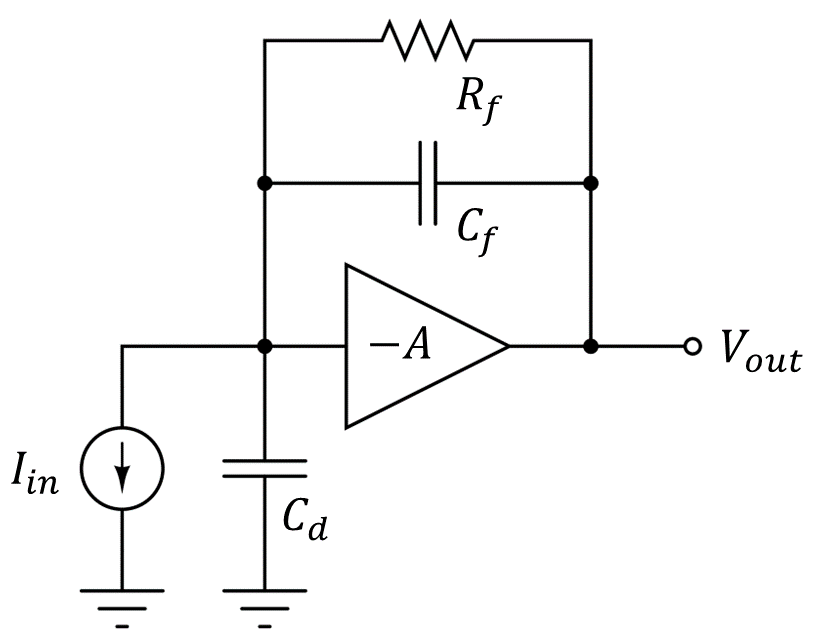
\includegraphics[width=\linewidth]{images/eq_model.png}
    \caption{Principe de base d'un feedback TIA.}
    \label{fig:eq_model}
\end{wrapfigure}

Pour faire la conception de notre préamplificteur, nous avons fait une recherche bibliographique sur les amplificateurs de transimpédance, et sur les front-end de détection. Les publications \cite{razavi_2000}, \cite{razavi_2019} et \cite{razavi_2023} nous ont permis de comprendre le principe de la conception des TIA. Cela nous a donné l'idée d'utiliser un amplificateur de tension contre-réactionné.

En outre, la publication \cite{sansen_1990} nous a aidé pour se familiariser avec les préamplificateurs bas bruit à base de CMOS, et comment utiliser comme impédance de contre-réaction une capacité en parallèle à une résistance, pour contrôler la bande passante.

Le circuit utilisé est un système de premier ordre comme l'illustre la figure \ref{fig:eq_model}, dont la fonction de transfert de transimpédance est

\begin{equation}\label{eq:transfer}
    \frac{V_{out}}{I_{in}}=\frac{Z_{0}}{1+\j\frac{f}{f_{c}}}
    \quad
    \text{avec}
    \quad
    Z_{0}=\frac{AR_{f}}{A + 1}
    \quad
    \text{et}
    \quad
    f_c=\frac{A+1}{2\pi R_f(AC_f+C_f+C_d)}
\end{equation}


\FloatBarrier
\newpage
\section{Conception}\label{sec:conception}

\subsection{Topologie}

Le circuit final complet est représenté dans la figure \ref{fig:circuit_complet}. Dans l'amplificateur de tension du circuit final, nous avons trois étages de base. Le premier est une source commune, qui doit présenter le minimum de bruit possible, vu que c'est le primer transistor dans le chemin du signal. Le deuxième est une grille commune, qui constitue avec la source commune un cascode replié, qui fait l'amplification de tension. Et le troisième étage est un suiveur qui sert à diminuer l'impédance de sortie du circuit, et assurer la bonne polarisation en entrée et en sortie du cascode quand l'amplificateur est contre-réactionné. Le dimentionnement de ces trois transistors de base est en annexe.

Nous utilisons une source de courant parfaite pour alimenter les miroirs de courant qui polarisent le circuit.

Pour réaliser le feedback, nous utilisons une résistance $R_f$ que nous relions à la sortie du suiveur. Par contre, nous savons qu'en AC, le buffer ne change pas le signal, alors nous avons choisit de relier la capacité de feedback $C_f$ à la sortie du cascode replié, pour aider la capacité $C_y$ à garantir la stabilité.

\begin{figure}[htp!]
    \centering
    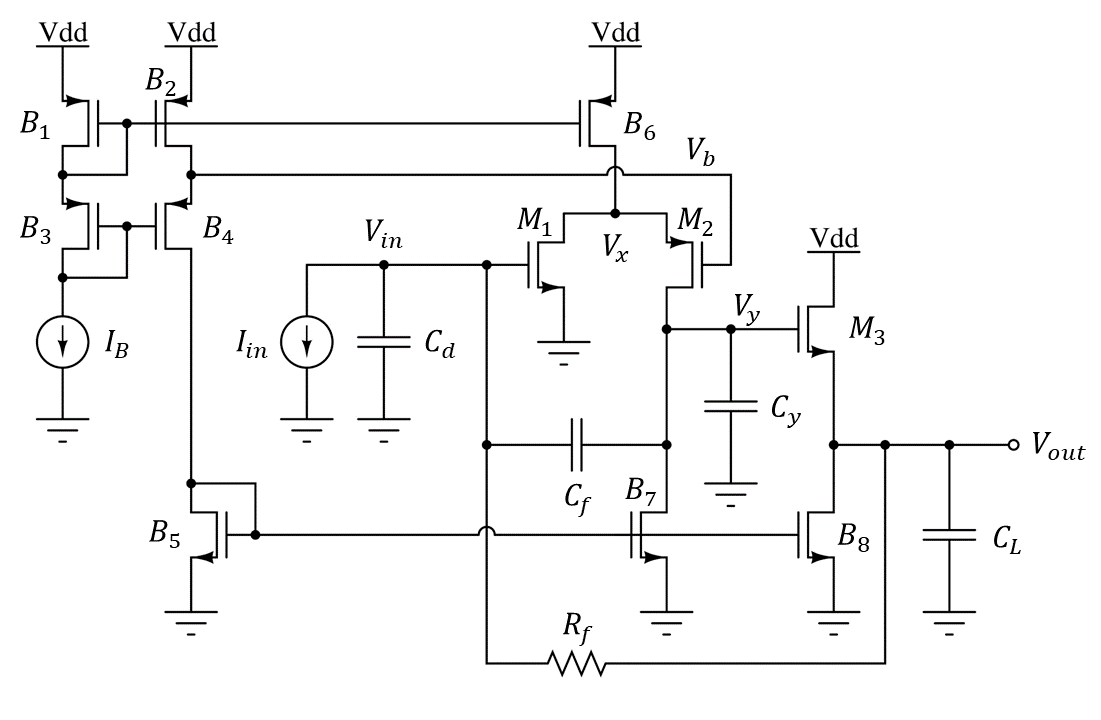
\includegraphics[width=\linewidth]{images/circuit_complet.png}
    \caption{Topologie du circuit final réalisé.}
    \label{fig:circuit_complet}
\end{figure}

\begin{table}[htp!]
\centering
\resizebox{\textwidth}{!}{%
\begin{tabular}{|c|c|c|c|c|c|c|c|c|c|c|c|}
\hline
\rowcolor[HTML]{CDCDCD} 
                                       & \textbf{$M_1$}              & \textbf{$M_2$}              & \textbf{$M_3$}                & \textbf{$B_1$}                & \textbf{$B_2$}                & \textbf{$B_3$}                & \textbf{$B_4$}                & \textbf{$B_5$}                & \textbf{$B_6$}                & \textbf{$B_7$}               & \textbf{$B_8$}                \\ \hline
\cellcolor[HTML]{CDCDCD}\textbf{$W$}   & $\sis{1}{\milli\meter}$     & $\sis{300}{\micro\meter}$   & $\sis{25}{\micro\meter}$      & $\sis{400}{\nano\meter}$      & $\sis{400}{\nano\meter}$      & $\sis{500}{\micro\meter}$     & $\sis{500}{\micro\meter}$     & $\sis{10}{\micro\meter}$      & $\sis{13}{\micro\meter}$      & $\sis{135}{\micro\meter}$    & $\sis{105}{\micro\meter}$     \\ \hline
\cellcolor[HTML]{CDCDCD}\textbf{$L$}   & $\sis{350}{\nano\meter}$    & $\sis{350}{\nano\meter}$    & $\sis{350}{\nano\meter}$      & $\sis{1}{\micro\meter}$       & $\sis{1}{\micro\meter}$       & $\sis{1}{\micro\meter}$       & $\sis{1}{\micro\meter}$       & $\sis{1}{\micro\meter}$       & $\sis{1}{\micro\meter}$       & $\sis{1}{\micro\meter}$      & $\sis{1}{\micro\meter}$       \\ \hline
\cellcolor[HTML]{CDCDCD}\textbf{$g_m$} & $\sis{6.4}{\milli\siemens}$ & $\sis{2.1}{\milli\siemens}$ & $\sis{1.192}{\milli\siemens}$ & $\sis{12.81}{\micro\siemens}$ & $\sis{12.81}{\micro\siemens}$ & $\sis{213.1}{\micro\siemens}$ & $\sis{212.8}{\micro\siemens}$ & $\sis{129.6}{\micro\siemens}$ & $\sis{479.2}{\micro\siemens}$ & $\sis{1.78}{\milli\siemens}$ & $\sis{1.356}{\milli\siemens}$ \\ \hline
\end{tabular}%
}
\caption{Tableau avec toutes les valeurs des transistors illustrés à la figure \ref{fig:circuit_complet}.}
\label{tab:transistor_values}
\end{table}

\FloatBarrier

\subsection{Projet Initiale}

Nous voulons un gain $A$ élevé pour pouvoir simplifier \eqref{eq:transfer} en \eqref{eq:simplified}.

\begin{equation}\label{eq:simplified}
    Z_{0}\approx R_f
    \quad
    \text{et}
    \quad
    f_c\approx\frac{1}{2\pi R_fC_f}
\end{equation}

On choisit $R_f=\sis{5}{\kilo\ohm}$ et $C_f=\sis{630}{\femto\farad}$, ce qui nous donne une transimpédance $Z_0\approx\sis{5}{\kilo\ohm}$ et une fréquence de coupure $f_c\approx\sis{50.5}{\mega\hertz}$. Pour commencer la conception de l'amplificateur de tension, nous avons réalisé un dimensionnement initial qui ne respectait pas forcément l'intégralité du cahier de charge. Comme le transistor $M_1$ est celui qui contribue le plus au bruit en entrée, on commence par définir quel $g_m$ on veut pour le transistor. La relation entre le bruit et $g_m$ est exprimée en \eqref{eq:noise_m1}.

\begin{equation}\label{eq:noise_m1}
    e_{ni}^{RMS}\approx\sqrt{\frac{4kT\gamma_{M1}}{g_{mM1}}}
\end{equation}

On choisit un $g_{mM1}$ de l'ordre de $\sis{10}{\milli\siemens}$, ce qui se traduit par un bruit $e_{ni}^{RMS}$ de l'ordre de $\sis{1}{\nano\volt\per\sqrt{\hertz}}$.

Après cela, nous avons mis à l'échelle le transistor $M_2$ pour obtenir un gain global de $\sis{60}{\decibel}$, en utilisant \eqref{eq:gm_m2} et \eqref{eq:cg_gain}.

\begin{equation}\label{eq:gm_m2}
    g_{mM2}=2\sqrt{K_p\frac{W_{M2}}{L_{M2}}I_{DM2}}
\end{equation}

\begin{equation}\label{eq:cg_gain}
    A_{GC}=\num{1.2}\cdot g_{mM2}\left(r_{dsB7}//r_{dsM2}\right)
\end{equation}

Comme un suiveur a un gain d'environ $\sis{-2}{\decibel}$, notre amplificateur de tension doit avoir un gain total de $\sis{58}{\decibel}$.

Pour polariser les transistors $M_1$, $M_2$ et $M_3$, on utilise des transistors $B_1$ à $B_8$ configurés en miroirs de courant et source de tension. Nous choisissons $B_1=B_2$ et $B_3=B_4$, tous avec $L=\sis{1}{\micro\meter}$.

Pour polariser la grille du transistor $M_2$, nous fixons $W_{B1}=W_{B2}=\sis{400}{\nano\meter}$ et paramétrons $W_{B3}=W_{B4}$ pour déterminer $ V_b$. Pour obtenir $V_b\approx\sis{1}{\volt}$, tension définie pour le dimensionnement de $M_2$, on trouve $W_{B3}=W_{B4}=\sis{500}{\micro\meter}$.

\subsection{Étapes de Validation}

Une fois la conception initiale terminée, nous commençons à vérifier chaque spécification dans le livre de charge. Nous commençons par la stabilité. En effectuant des simulations temporelles et de stabilité, nous avons constaté que le circuit oscillait considérablement. Pour remédier à ce fait, nous plaçons un condensateur $C_y$ entre le cascode replié et le suiveur. Nous arrivons à la valeur $C_y=\sis{10}{\femto\farad}$, que nous implémentons avec 3 condensateurs $\sis{30}{\femto\farad}$ en série.

Notre circuit est stable, avec un faible bruit d'entrée et un bon gain en boucle ouverte. Le problème maintenant est que le circuit consomme trop. Pour remédier à ce problème, nous paramétrons le courant de polarisation $I_b$ et traçons la puissance consommée en fonction de $I_b$. Nous avons vérifié que pour ne pas dépasser $\sis{2}{\milli\watt}$, nous devons limiter $I_b$ en $\sis{8.8}{\micro\ampere}$.

Comme nous avons diminué les courants de polarisation de $M_1$, $M_2$ et $M_3$, nous avons recalculé le rapport d'aspect de chaque transistor en utilisant \eqref{eq:wl_updater} pour garantir le même $g_m$.

\begin{equation}\label{eq:wl_updater}
    \frac{W}{L}=\frac{g_m^2}{4K_{n,p}I_D}
\end{equation}

Au cours du processus de mise en page, nous avons dû modifier la configuration du transistor $M_1$. Pour mieux répartir les composants dans le circuit, nous avons implémenté $M_1$ avec 40 transistors identiques en parallèle. Cette modification est prise en compte dans les simulations de la section \ref{sec:simulations}.

\FloatBarrier
\newpage
\section{Résultats de Simulation}\label{sec:simulations}

Pour simuler le circuit, nous avons créé un sous-circuit avec uniquement les composants qui font réellement partie de notre amplificateur. Ce sous-circuit peut être vu dans la figure \ref{fig:csh_final}. Après cela, nous avons créé un symbole pour le sous-circuit que nous avons utilisé dans un circuit de testbench pour exécuter toutes les simulations. Le circuit de testbench est visible sur la figure \ref{fig:sch_bench}.

\begin{figure}[htp!]
    \centering
    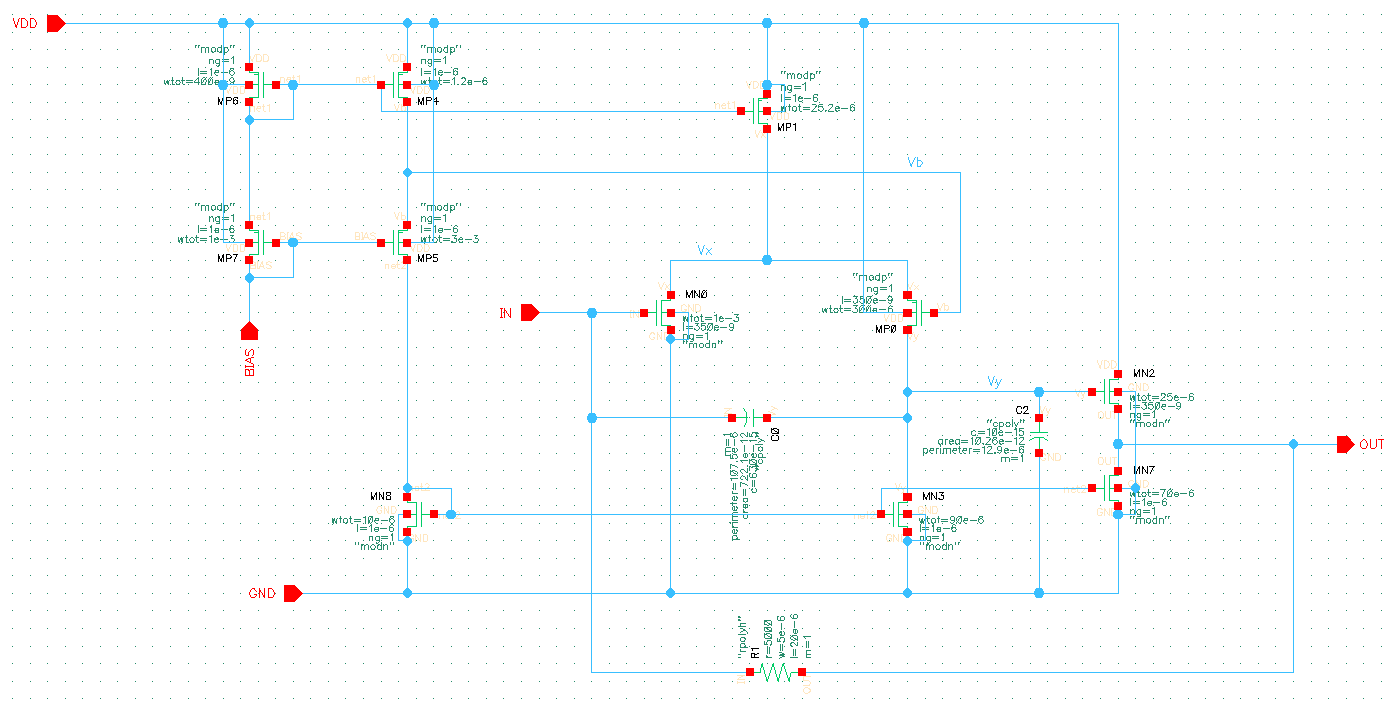
\includegraphics[width=\linewidth]{images/csh_final.png}
    \caption{Schéma de la version finale de l'amplificateur.}
    \label{fig:csh_final}
\end{figure}

\begin{figure}[htp!]
    \centering
    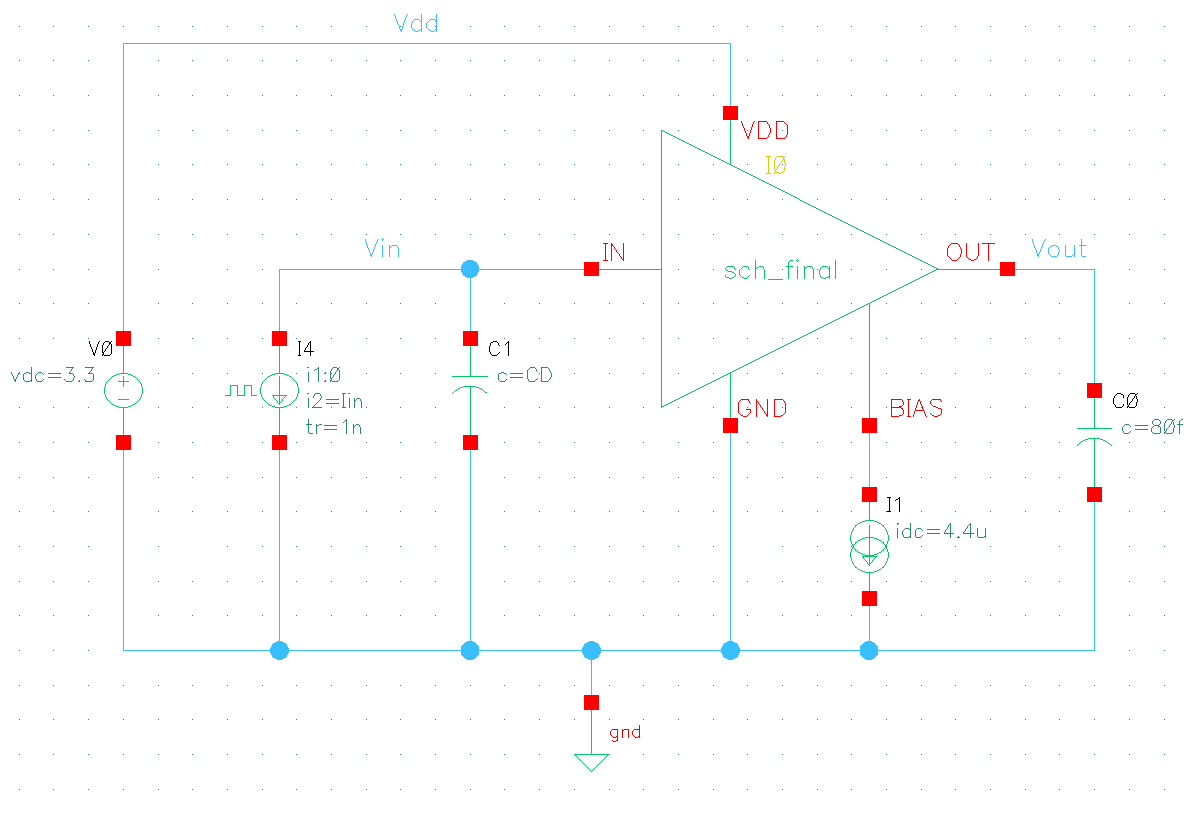
\includegraphics[width=0.7\linewidth]{images/sch_bench.png}
    \caption{Schéma du testbench utilisé pour les simulations.}
    \label{fig:sch_bench}
\end{figure}


\subsection{Simulation Temporelle - Conditions Nominales}

D'abord, nous effectuons la simulation temporelle pour vérifier que le système est stable pour les extrêmes de notre dynamique d'entrée. Cette simulation nous permet aussi de vérifier si nous respectons le taux de comptage. Pour cela, on se place dans le cas extrême où nous avons chaque deux impulsions successives sont séparées de \sis{50}{\nano\second}. La figure \ref{fig:tran} représente le résultat de cette simulation. Nous observons que la sortie du système est capable de se stabiliser dans la \textit{baseline} avant l'arrivée de l'impulsion suivante. La dynamique de sortie (crête d'impulsion) est comprise entre \sis{502.03}{\milli\volt} et \sis{1.0859}{\volt}. Et la \textit{baseline} est de \sis{500}{\milli\volt}.

\begin{figure}[htp!]
    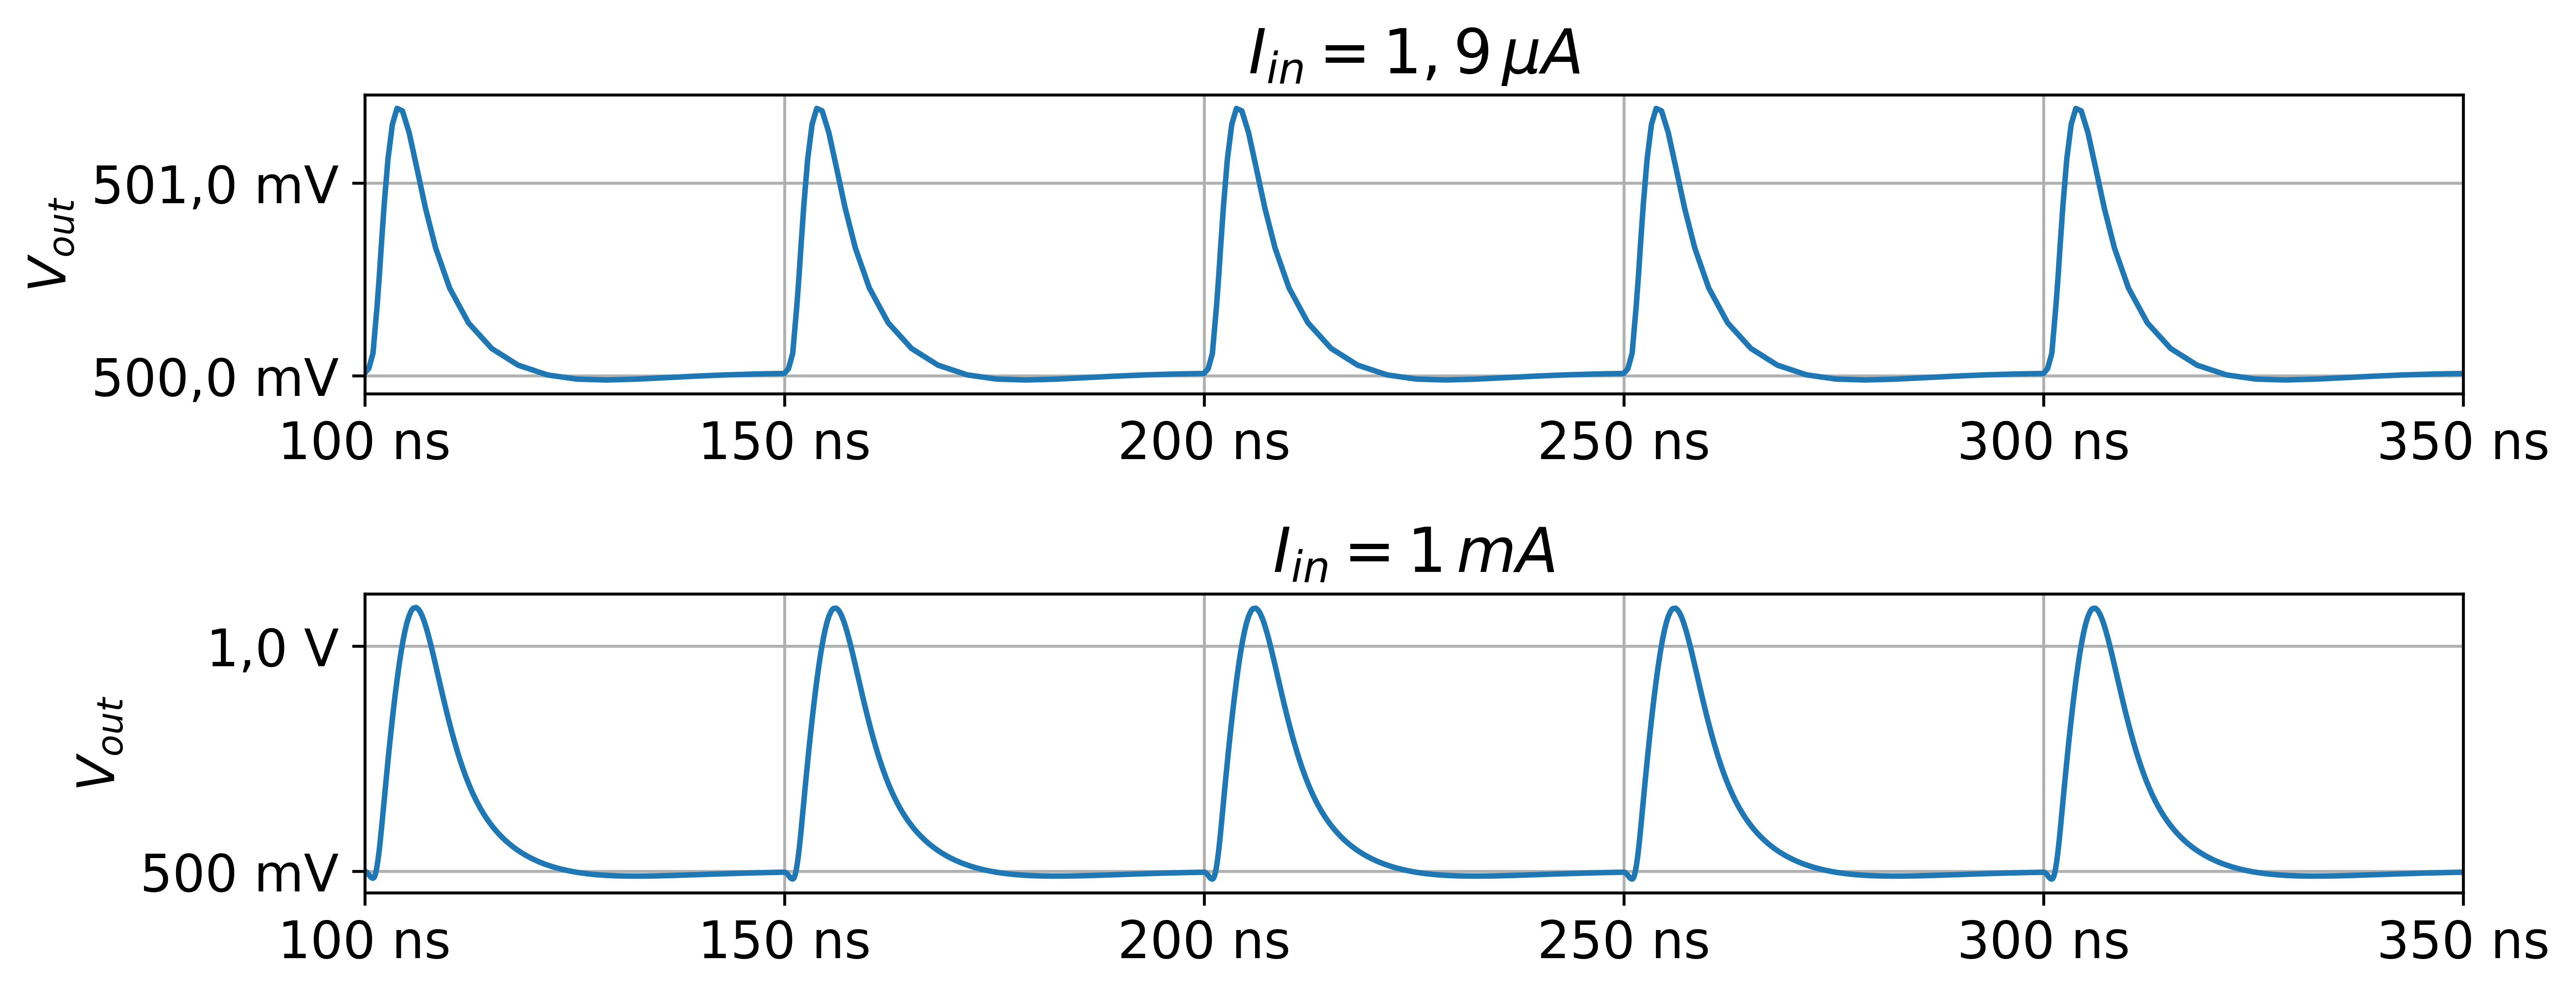
\includegraphics[width=\linewidth]{images/tran.png}
    \caption{Simulation Temporelle pour les extrêmes de la dynamique d'entrée.}
    \label{fig:tran}
    \centering
\end{figure}

\subsection{Simulation Temporelle - Diverses Capacités de Capteur}

Dans cette partie, nous étudions l'effet du changement de la capacité du détecteur sur la réponse du système. Pour cela, nous choisissons trois valeurs différentes de $C_d$, et nous faisons la simulation pour les valeurs extrêmes de l'entrée. La figure \ref{fig:tran_cd_sweep} représente les différents résultats obtenus. Dans cette simulation, nous avons une période de \sis{100}{\nano\second}, pour voir si le système ce stabilise. Nous remarquons que pour $C_d = \sis{18}{\pico\farad}$ le système prend plus que \sis{50}{\nano\second} pour se stabiliser. Mais il se stabilise quand même. Nous remarquons aussi que la dynamique en sortie diminue en augmentant la valeur de $C_d$.

\begin{figure}[htp!]
    \centering
    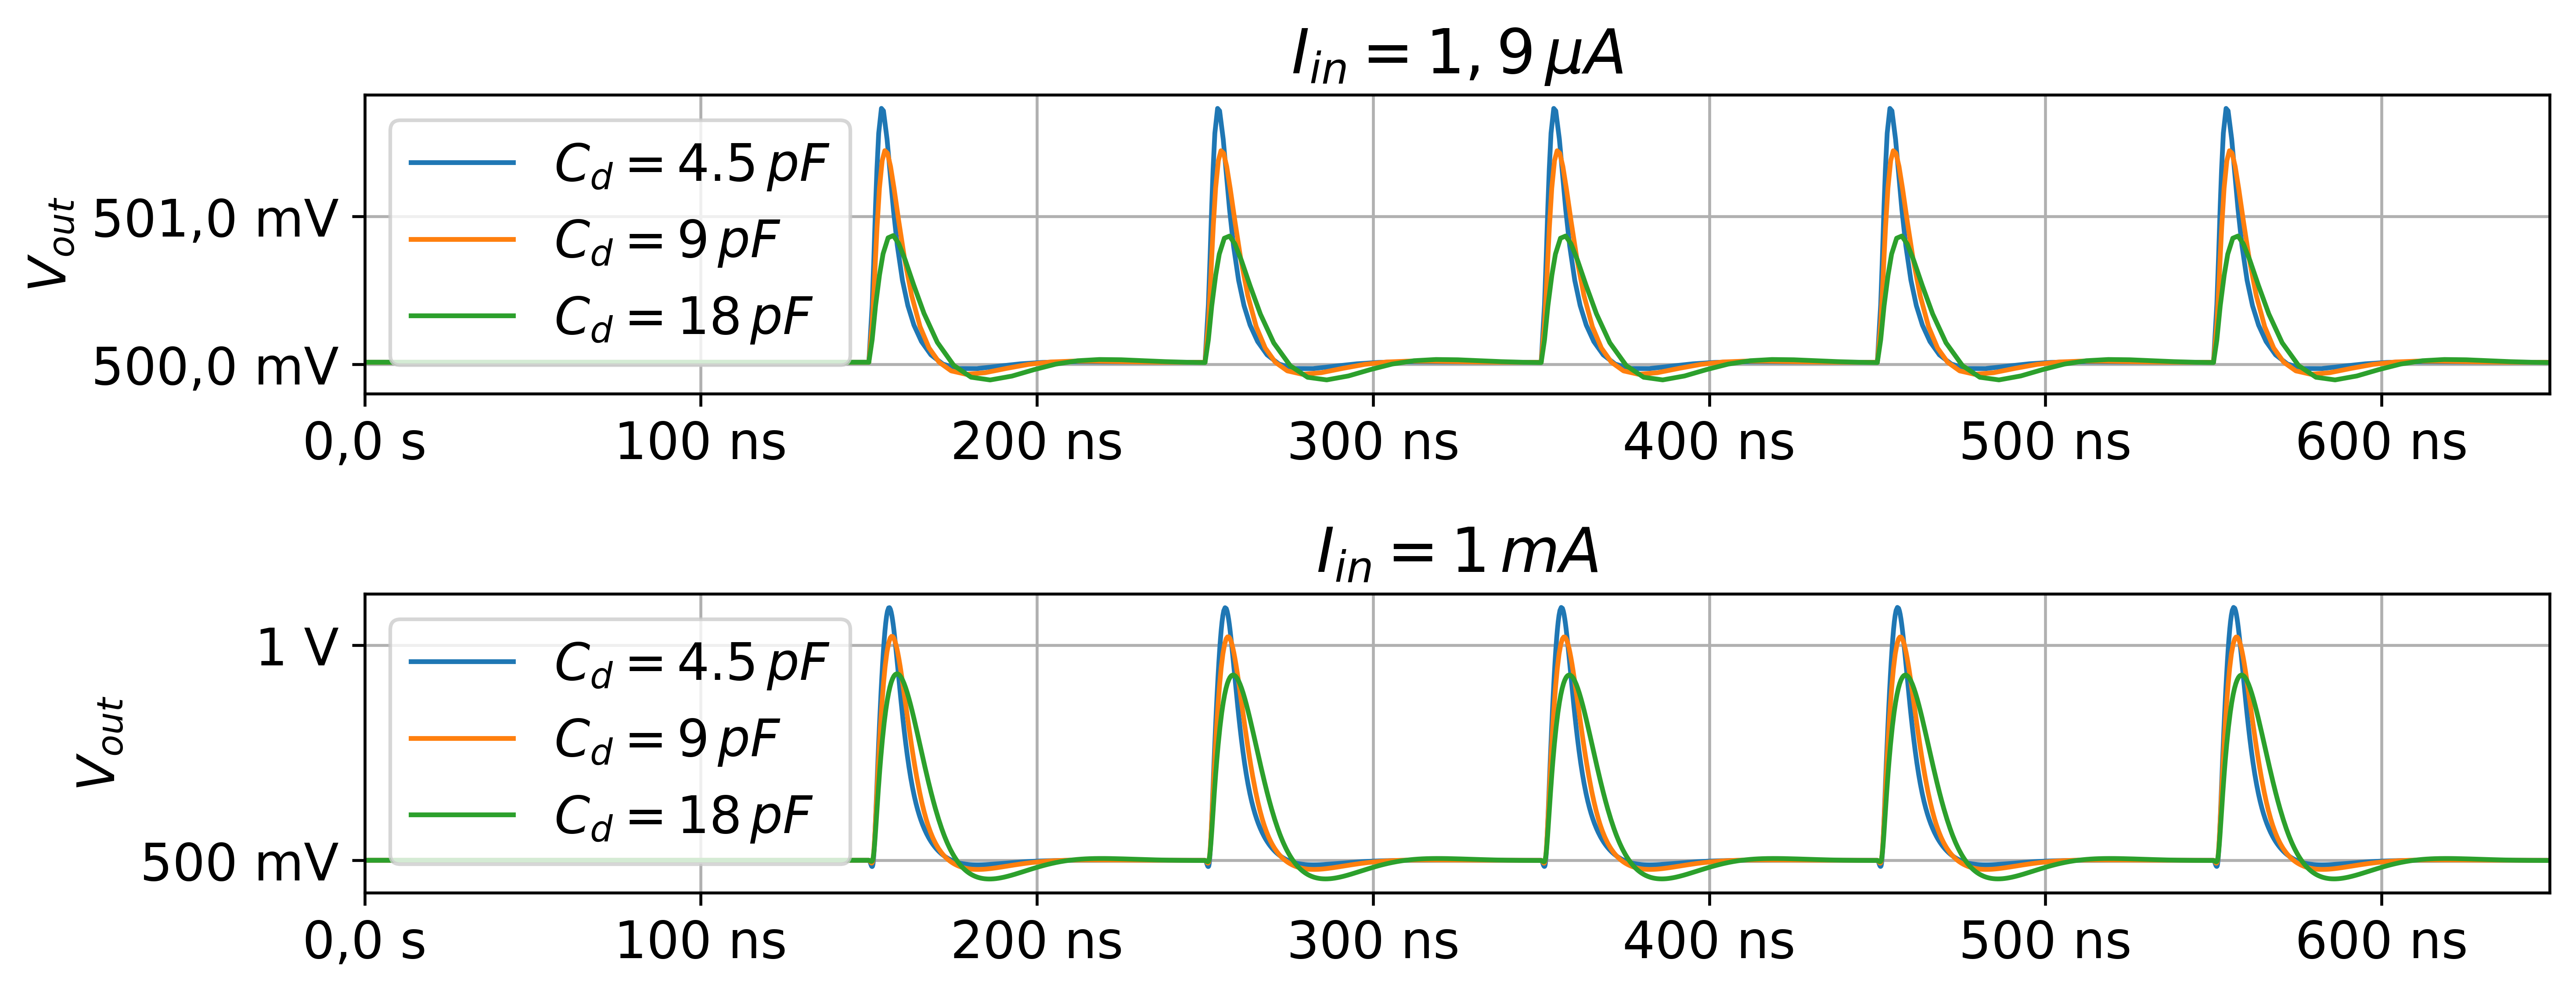
\includegraphics[width=\linewidth]{images/tran_cd_sweep.png}
    \caption{Simulation Temporelle pour différentes valeurs de la capacité du capteur.}
    \label{fig:tran_cd_sweep}
\end{figure}

\subsection{Simulation Temporelle - Diagramme de l'Œil}

Dans cette partie, nous simulons le diagramme de l'œil pour $I_{in}$ minimal, avec une simulation temporelle avec bruit. Nous obtenons le diagramme représenté dans la figure \ref{fig:eye_diagram}, qui monte que malgré l'existence du bruit, nous arrivons bien à détecter l'impulsion de sortie même avec la plus petite valeur en entrée.

\begin{figure}[htp!]
    \centering
    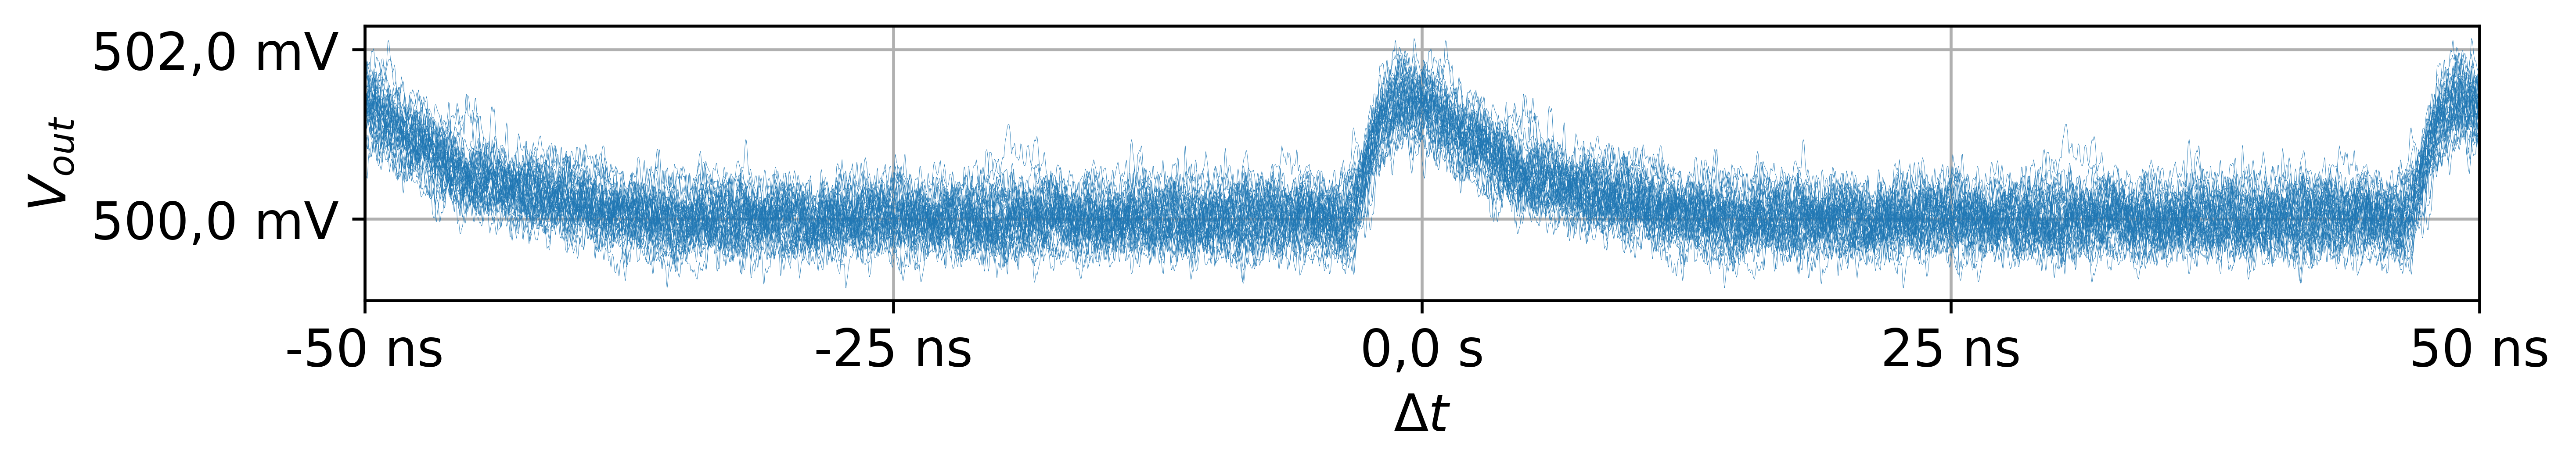
\includegraphics[width=\linewidth]{images/eye_diagram.png}
    \caption{Diagramme de l'œil pour l'entrée minimale.}
    \label{fig:eye_diagram}
\end{figure}


\subsection{Réponse Fréquentielle - Boucle Ouverte}

Nous réalisons la simulation AC en boucle ouverte pour extraire la valeur du gain de tension $A$ de l'amplificateur, et aussi pour vérifier la stabilité du système, en mesurant la marge de gain et la marge de phase. On obtient un gain en tension de $A=\sis{57.554}{\decibel}$, une valeur proche de la valeur théorique de $\sis{58}{\decibel}$. Nous avons aussi une marge de phase de \ang{70.1807}, et une marge de gain de \sis{18.6734}{\decibel}. Donc le système est bien stable.

\begin{figure}[htp!]
    \centering
    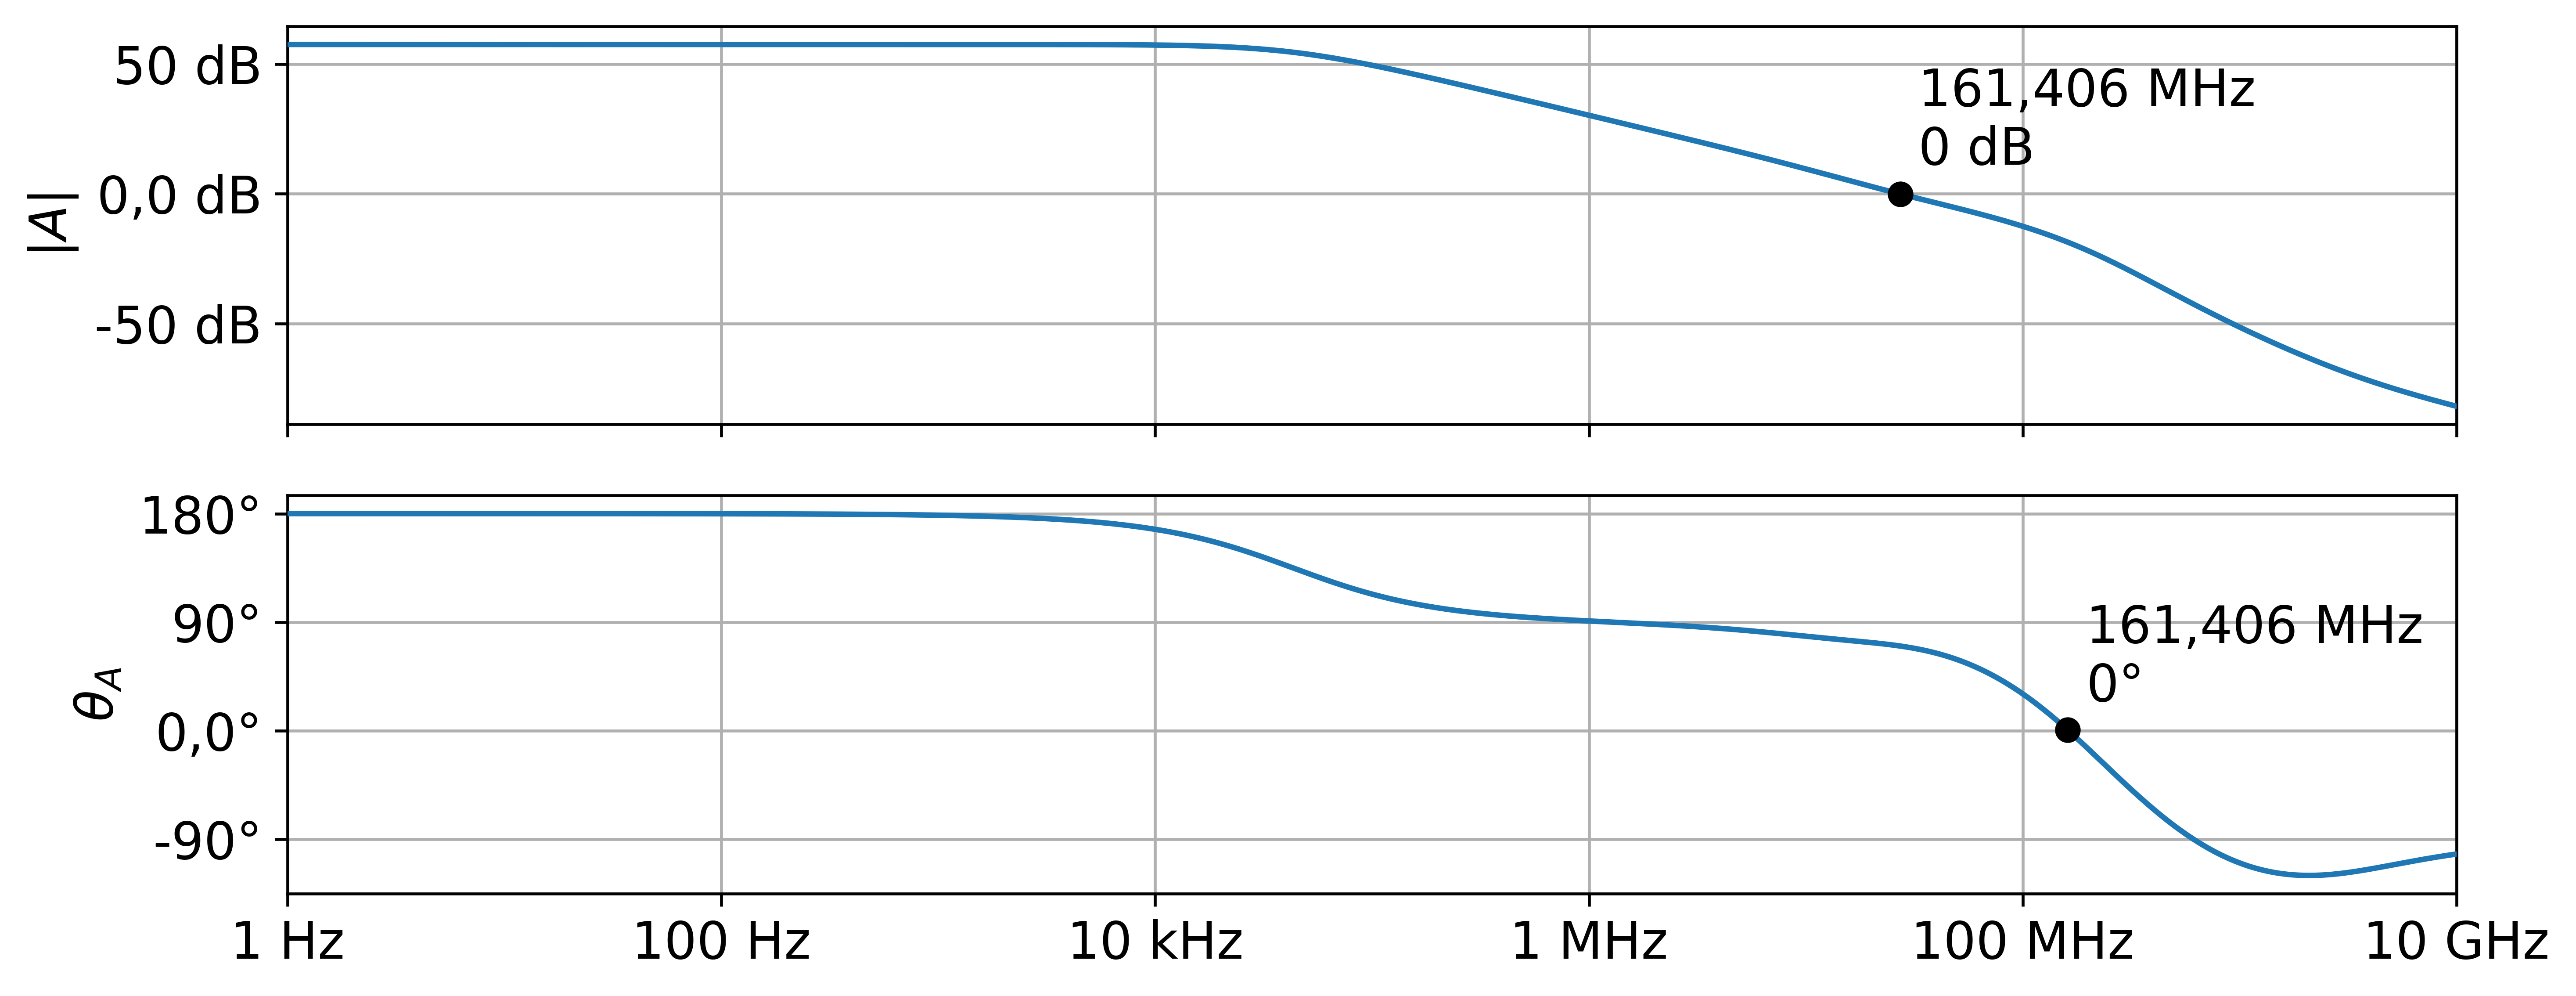
\includegraphics[width=\linewidth]{images/open_loop.png}
    \caption{Réponse en boucle ouverte. Les marqueurs indiquent les points de \sis{0}{\decibel} et d'inversion de phase.}
    \label{fig:open_loop}
\end{figure}


\subsection{Réponse Fréquentielle - Boucle Fermée}

Après vérification du comportement en boucle ouverte du circuit, nous fermons la boucle pour vérifier la vraie réponse fréquentielle du système. Nous obtenons les résultats représentés dans la figure \ref{fig:gain_transimp}, qui donnent le gain de transimpédance. Théoriquement, nous avons $Z_0 = \sis{4.9934}{\kilo\ohm}$, et la simulation donne $Z_0 = \sis{5.01146}{\kilo\ohm}$, et ce sont deux valeurs très proches. Pour la fréquence de coupure, nous obtenons théoriquement la valeur de fréquence $f_c = \sis{50.052}{\mega\hertz}$, et la simulation donne $f_c = \sis{41.1019}{\mega\hertz}$, ces valeurs sont un peu différentes, mais c'est normal puisque la première approche théorique ne prend pas en considération la caractéristique passe bas de l'amplificateur de tension.  

\begin{figure}[htp!]
    \centering
    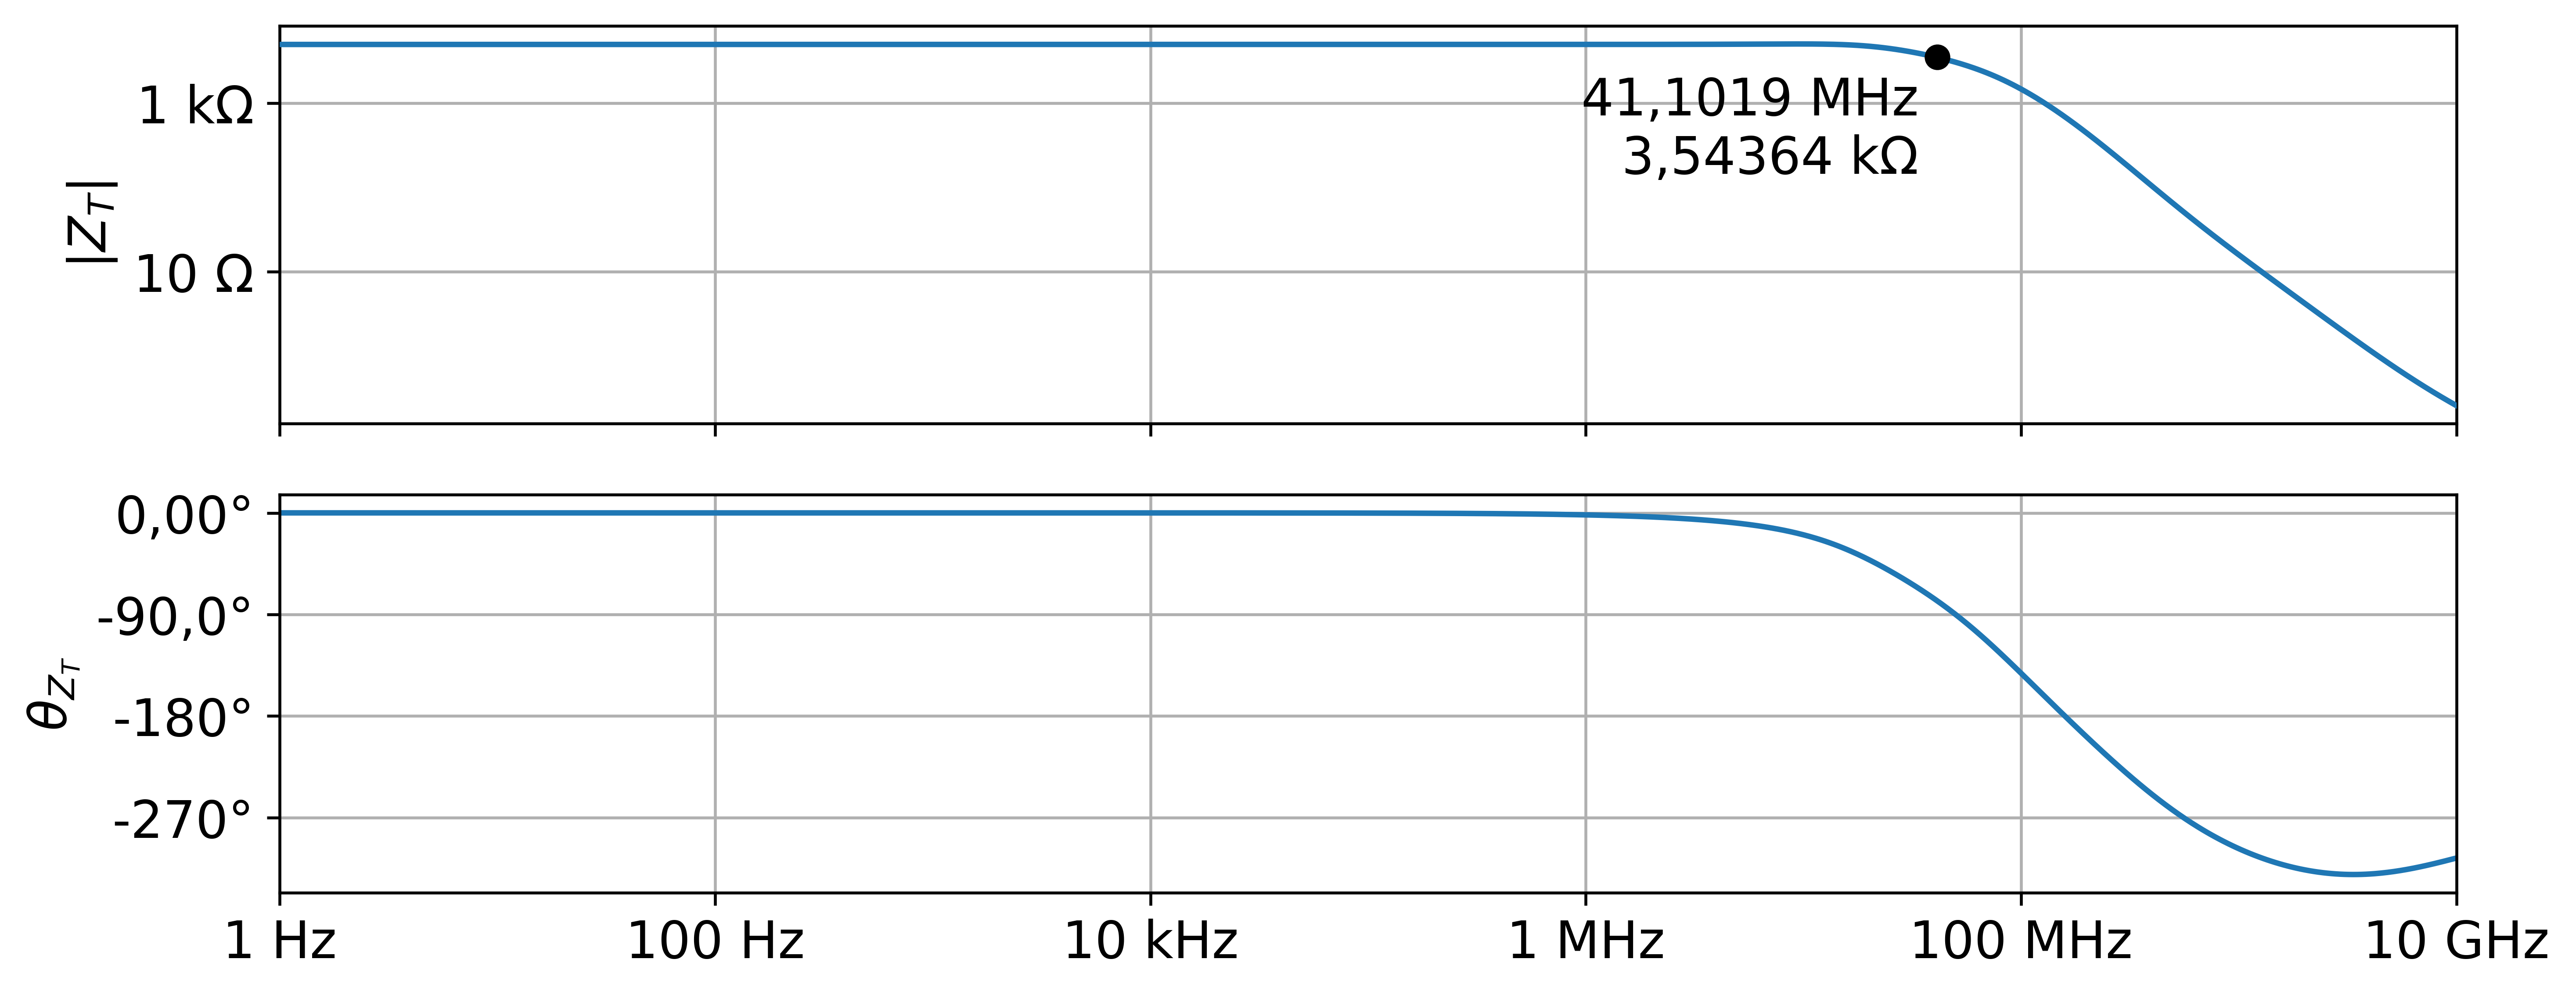
\includegraphics[width=\linewidth]{images/gain_transimp.png}
    \caption{Réponse en boucle fermée. Le marqueur indique la fréquence de coupure.}
    \label{fig:gain_transimp}
\end{figure}

\subsection{Densité Spectrale du Bruit}

Nous lançons la simulation \aspas{noise} entre \sis{1}{\hertz} et \sis{10}{\giga\hertz}, et nous traçons la densité spectrale du bruit en entrée. Et nous utilisons cette courbe pour tracer le bruit RMS d'entrée, en passant les données dans un calculateur et on mesurant le bruit intégré en fonction de la fréquence limite supérieure d'intégration. Nous obtenons les résultats présentés dans la figure \ref{fig:input_noise}, qui montrent que le bruit critique correspond à \sis{1000}{\electron} est atteint à partie de la fréquence \sis{227.214}{\mega\hertz}, qui est une valeur très supérieure à notre fréquence équivalente du bruit,\endnote{

Supposons que nous ayons un système avec une fonction de transfert \eqref{eq:transfer_real}. 

\begin{equation}\label{eq:transfer_real}
    H(f)=\frac{H_0}{1+\j\frac{f}{f_c}}
\end{equation}

Nous pouvons définir un système équivalent de bruit blanc plus facile à utiliser pour les calculs de fonction de transfert \eqref{eq:transfer_equivalent}.

\begin{equation}\label{eq:transfer_equivalent}
    H_{eq}(f)=
    \begin{cases}
        H_0 & \quad\text{si}\quad\abs{f}\leq f_{eq}\\
        0   & \quad\text{si}\quad\abs{f}>f_{eq}
    \end{cases}
\end{equation}

Afin d'obtenir le paramètre $f_{eq}$ du filtre équivalent, nous devons nous assurer que le bruit intégré pour les deux filtres est le même. Cette condition est exprimée mathématiquement en \eqref{eq:noise_equation}.

\begin{equation}\label{eq:noise_equation}
    \int_{-\infty}^{\infty}e_{ni}^2\abs{H(f)}^2df=\int_{-\infty}^{\infty}e_{ni}^2\abs{H_{eq}(f)}^2df
\end{equation}

En résolvant \eqref{eq:noise_equation} nous obtenons la relation $f_{eq}=\frac{\pi}{2}f_c$.

} qui est au alentour de \sis{64.6}{\mega\hertz}.

\begin{figure}[htp!]
    \centering
    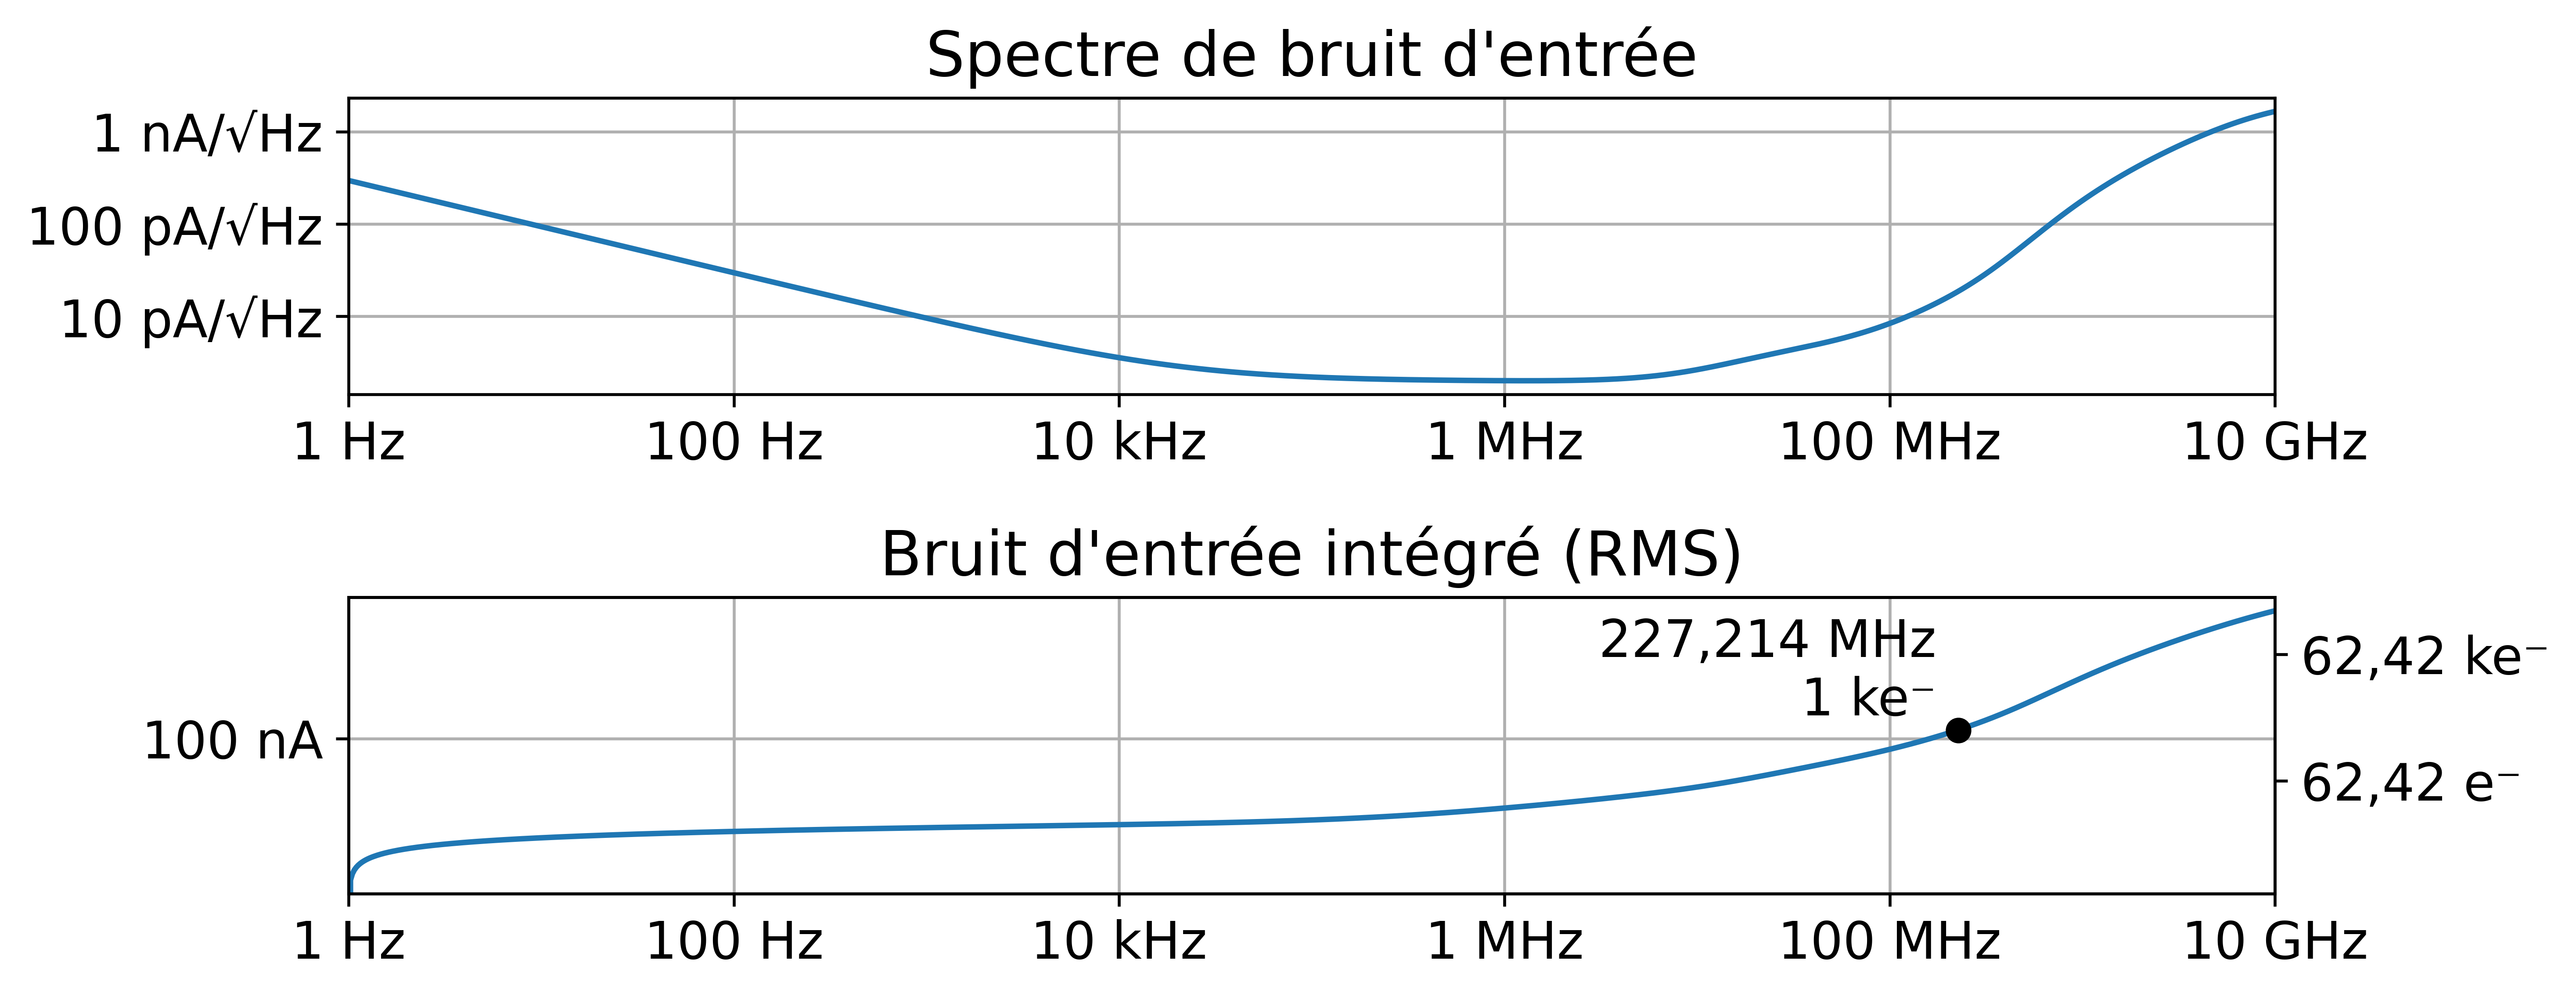
\includegraphics[width=\linewidth]{images/input_noise.png}
    \caption{Bruit ramenée en entrée. Le marqueur montre dans quelle mesure nous pouvons intégrer et toujours respecter la spécification de bruit.}
    \label{fig:input_noise}
\end{figure}

\subsection{Linéarité}

Nous avons lancé une simulation temporelle pour plusieurs valeurs d'amplitudes d'entrée (31 valeurs de $I_{in}$), et nous avons tracé la courbe représentative de la valeur de crête de la tension de sortie, en fonction de celle du courant d'entrée. Nous obtenons les résultats représentes dans la figure \ref{fig:lin_test}, qui montre que le système est linéaire.

Nous avons tracé la droite de régression linéaire avec l'équation $V_{out}=aI_{in}+b$ avec $a=\sis{584.499}{\ohm}$ et $b=\sis{524.616}{\milli\volt}$. Nous avons calculé le coefficient de détermination linéaire $r^2=\num{0.99557}$, et c'est une valeur très proche à l'unité, donc on peut dire que le système présente un degré important de linéarité. Mais pour être sûr, nous mesurons la valeur absolue de la différence entre les données et la courbe de régression. Cette valeur est exprimée en pourcentage par rapport à la dynamique en sortie. Nous remarquons que l'erreur maximale est de $\delta_{max}=\num{4.06}\%$. 


\begin{figure}[htp!]
    \centering
    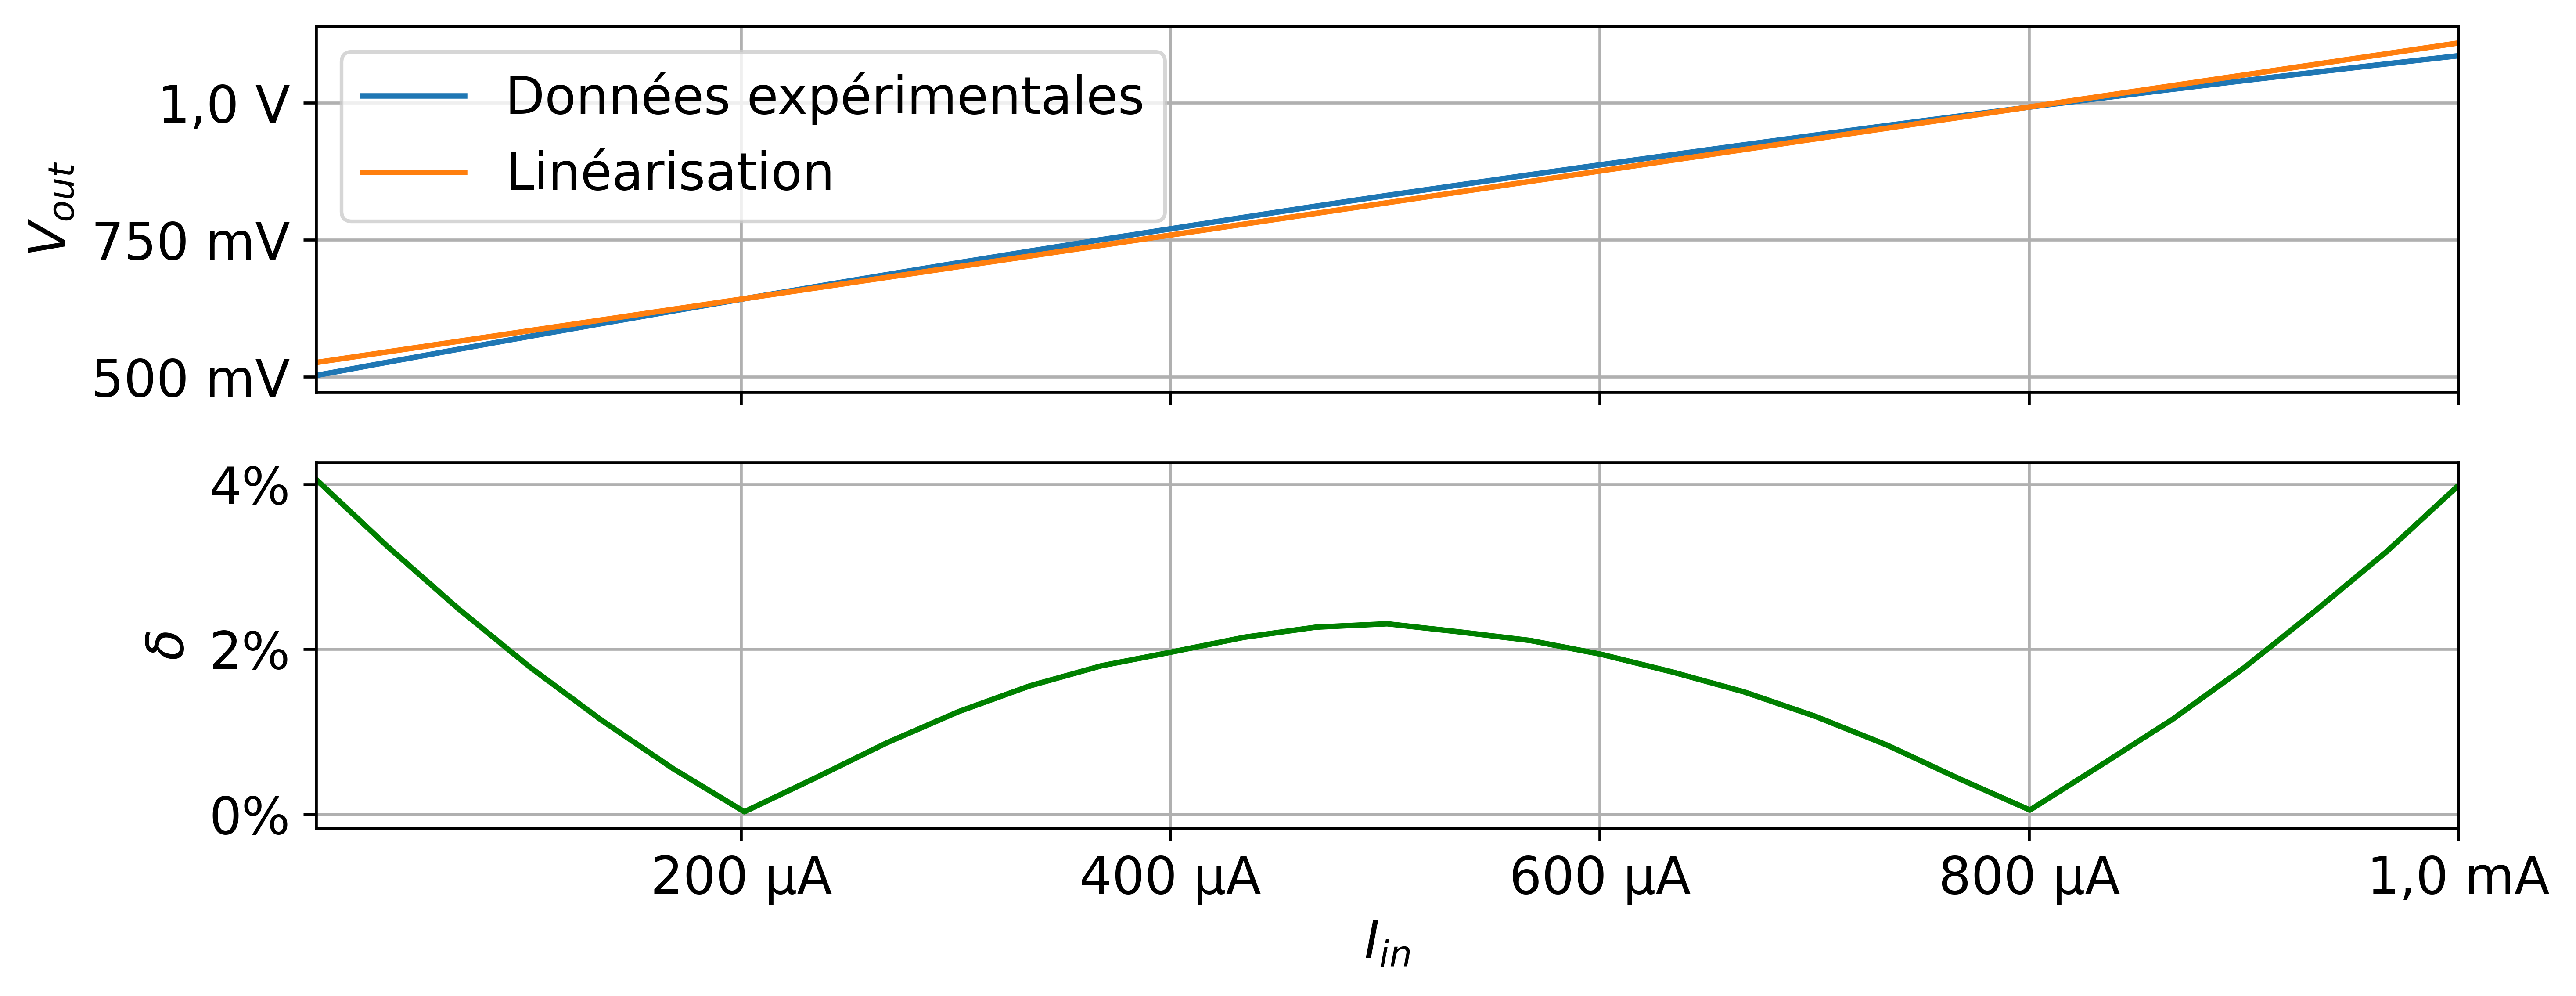
\includegraphics[width=\linewidth]{images/lin_test.png}
    \caption{Simulation de linéarité.}
    \label{fig:lin_test}
\end{figure}

\subsection{Consommation}

Pour la consommation, nous respectons bien le cahier des charges, puisque le circuit consomme entre \sis{1.68203}{\milli\watt} pour $I_{in}=\sis{1.9}{\micro\ampere}$ et \sis{1.7297}{\milli\watt} pour $I_{in}=\sis{1}{\milli\ampere}$.

\begin{figure}[htp!]
    \centering
    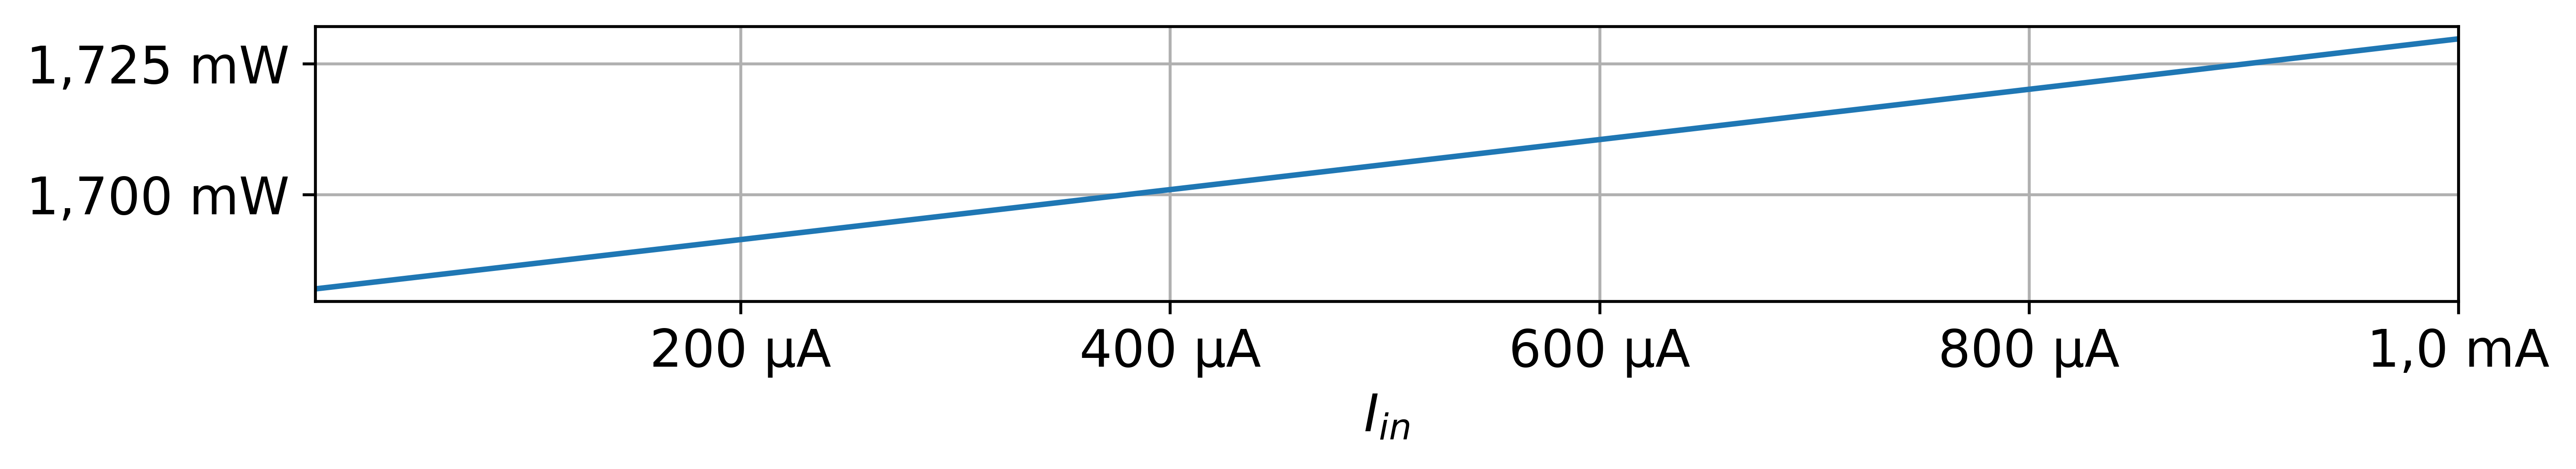
\includegraphics[width=\linewidth]{images/power.png}
    \caption{Simulation de consommation.}
    \label{fig:power}
\end{figure}

\FloatBarrier
\newpage
\section{Layout}

Après avoir validé le fonctionnement de notre circuit, nous avons commencer à faire le layout du sous-circuit, et nous avons finis tout le routage nécessaire. Cela nous a permis de découvrir plein de fonctionnalités de cadence, et d'acquérir les compétences techniques nécessaires pour faire le routage.

Enfin, nous avons lancé le test DRC (\textit{Design Rule Check}), et nous avons trouvé qu'il y a des petits problèmes dans notre layout, mais malheureusement, nous n'avons pas eu le temps pour corriger tous ces erreurs. Le problème est sur un objet spécifique qui est invisible et non modifiable. Il semble qu'il s'agisse d'un type de contrainte spécifique définie par le PDK (\textit{Process Design Kit}) de AMS que nous n'avons pas pu résoudre. Nous avons lancé aussi le test LVS (\textit{Layout Versus Schematic}), et nous n'avons pas trouvé d'erreurs, donc la correspondance entre notre layout et le circuit est bien vérifiée. La figure \ref{fig:layout_fig} montre le résultat du travail fait pour réaliser le dessin des masques.

\begin{figure}[htp!]
    \centering
    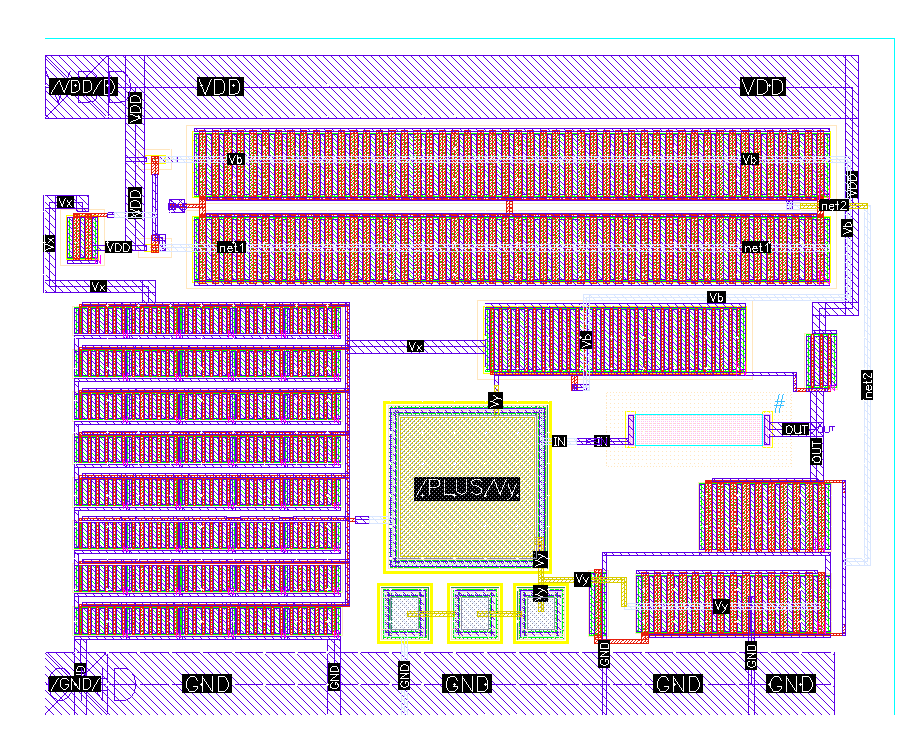
\includegraphics[width=\linewidth]{images/layout_fig.png}
    \caption{Layout du circuit final.}
    \label{fig:layout_fig}
\end{figure}

\FloatBarrier
\newpage
\section{Conclusion}

En guise de conclusion, nous pouvons dire que nous avons réussi ce projet, vu que notre circuit conçu répond bien au cahier des charges, et les différentes simulations effectuées montrent cela. 

Ce projet nous a permis d'acquérir des méthodes et des compétences nécessaires pour la conception d'un circuit en prennant en compte son cahier des charges et la durée limitée du projet, et nous a permis de se familiariser avec l'utilisation de l'outil cadence. C'était aussi l'opportunité pour nous de lier entre le cours théoriques (conception des circuits intégrés analogiques, circuits actifs hyperfréquences et optoélectroniques, etc...). En effet, nous avons exploité les relations et les connaissances déjà acquises pour faire la conception, comprendre les problèmes rencontrés, et améliorer le fonctionnement du circuit.

Enfin, nous remercions nos profs encadrements, car ils nous ont beaucoup aidé. Et grâce à leurs explications et à leurs assistances, nous avons pu profiter au maximum de ce projet.

\FloatBarrier
\newpage
\section{Preuve de Compétence}

Dans cette section chaque membre du groupe explique les compétences validées lors de l'élaboration du projet.

\subsection{EL HADI, Asmae}

Ce projet m'a permis d'acquérir plusieurs compétences, vu que c'est un grand projet où toutes mes connaissances théoriques et en logiciel se chevauchent pour le réussir. 

D'abord, j'estime acquérir un niveau N2 pour la compétence \aspas{Concevoir ou réaliser des solutions techniques, théoriques ou expérimentales, permettant de répondre à un cahier des charges}. Premièrement, la section \ref{sec:conception}, en particulier dans la partie étape de validation, qui montre comment nous avons évaluer notre circuit pour savoir s'il répond au cahier des charges ou pas, et si notre solution technique est fonctionnelle. Et à la fin, nous avons réussi à concevoir un système qui fonctionne parfaitement comme prévu.

Ensuite, j'ai appuyé sur toutes mes connaissances acquises dans les cours, les TDs, et les TPs, comme le cours de \aspas{conception des circuits intégrés analogiques}, et le cours des \aspas{circuits actifs hyperfréquences et optoélectroniques}. Toutes ces connaissances ont permis la conception d'une solution purement technique. En outre, nous avons réussi à rendre le projet avant le délai, et nous avons bien avancé sur le projet jusqu'au point de réaliser le layout du circuit (même s'il y a le test DRC ne passe pas totalement).

Également, ce projet était l'opportunité pour moi pour se familiariser avec l'outil Cadence, qui est un outil indispensable dans la conception des circuits intégrés analogiques, et l'outil Python pour tracer les différentes courbes et effectuer les différents calculs pour avoir une présentation et un rapport propres. Enfin, le rapport réalisé clarifie très bien les démarches de la conception et de la validation de ce circuit, et les détails présentés permettent la réulitisabilité de notre solution.

Ensuite, j'estime acquérir le niveau N2 pour la compétence \aspas{Mettre en oeuvre une démarche de recherche fondamentale ou appliquée à des fins d'innovation}. En effet, ce projet m'a permis de construire un méthodologie de développement et de recherches, et la sous-section \ref{sub:principe_du_circuit} montre que nous avons fait beaucoup de recherches complémentaires qui nous ont permis d'identifier l'état d'art et les plans d'actions pour ce projet. En plus, notre solution technique est bien pertinente car elle répond au cahier des charges et fait la fonction préamplification avec un bas bruit et une fonction de transimpédance. En plus, j'ai bien contribué dans ce projet, nous étions deux, et nous étions toujours présents, nous avons tous les deux participé à la réalisation de toute les parties du projet (recherches, conception, simulations, rapport et présentation, etc...) chose qui nous a permis de respecter le délai et les contraintes imposées. En outre, ce rapport illustre une prospective par rapport aux verrous identifiés grâce à la réalisation l'état de l'art. Et il présente aussi les résultats trouvés, et il montre que notre solution est bien fonctionnelle, et la présentation du projet que nous avons faites montre que les professeurs et nos camarades apprécient le travail réalisé. 

Enfin, Victor et moi avons construit une très bonne équipe, nous étions cohérent et en accord sur tous les points, car nous avons réussi à surmonter vite les moments de désaccord. Nous avons profité de communiquer en français et en anglais vu que nous sommes des étudions internationaux. Donc nous avons réussit à créer un environnement international et interculturel, et coopérer dans un binôme en mode projet. 

\subsection{SABIÁ PEREIRA CARPES, Victor}

Tout au long de ce projet, j'ai pu développer mes compétences d'ingénieur, en utilisant des outils théoriques en lien avec les logiciels de conception utilisés.

Les principales compétences développées sont les suivantes:

\begin{itemize}
    \item\textbf{Concevoir ou réaliser des solutions techniques, théoriques ou expérimentales, permettant de répondre à un cahier des charges:} Au cours de ce projet, j'ai pu exploiter mes expériences précédentes de mes études au Brésil et ici à Phelma. Nous avons pu analyser correctement les résultats de la simulation et les utiliser pour modifier le circuit jusqu'à ce que nous ayons une solution fonctionnelle qui respecte le cahier de charges. Nous avons terminé le projet à temps et, même si nous n'avons pas pu faire de simulations post-layout, nous avons réussi à finir un layout électriquement équivalent à notre schéma. Pour vérifier chaque aspect de notre circuit, nous avons utilisé le type de simulations pertinentes et les bonnes méthodes mathématiques et théoriques.

    \item\textbf{Coopérer dans une équipe ou en mode projet:} Presque toutes les sections de travail ont été réalisées en binôme. Nous avons pu bien répartir le travail. Nous nous sommes organisés pour réaliser le dimensionnement de tous les transistors et nous avons fait les analyses ensemble. La partie que nous avons faite de manière plus indépendante était la préparation de la présentation. Pendant que j'écrivais des scripts \textit{python} pour tracer les résultats de la simulation, Asmae s'occupait de produire elle-même les diapositives. En fin de compte, nous avons pu travailler en synergie les uns avec les autres.

    \item\textbf{Travailler et communiquer en environnement international et interculturel:} Asmae et moi sommes des étudiants internationaux venant de différents coins du monde. En travaillant ensemble, nous avons eu l'opportunité de communiquer en anglais et en français. De plus, dans les moments de repos entre les séances de travail, nous avons eu plusieurs échanges culturels, parlant des similitudes et des différences de nos cultures (cultures brésilienne et marocaine) et de nos autres collègues (culture française).
\end{itemize}

En résumé, Asmae et moi avons pu utiliser nos connaissances théoriques des outils de conception pour mener à bien la conception et la validation d'un préamplificateur bas bruit. Nous avons pu coopérer efficacement et partager certaines de nos différentes cultures et langues les uns avec les autres.

% Endnotes
\newpage
\renewcommand{\thesection}{N}
\printendnotes[itemize]

% References
\sisetup{output-decimal-marker = {.}}
\bibliographystyle{IEEEtran}
\bibliography{references.bib}
\addcontentsline{toc}{section}{Références}

\end{document}